\documentclass{article}
\usepackage[final]{pdfpages}
\usepackage{amssymb}
\usepackage{xspace}
\usepackage{import}
\usepackage{natbib}
\usepackage[pdftex]{hyperref}
\usepackage{url}
%\newcommand{\K}{\ensuremath{\mathbb{K}}\xspace}

%\newcommand{\Kall}[3]{\kall{#1}{#2}{#3}}
%\import{}{./k2latex.mm.sty}
\import{}{./macros.sty}


\title{\K Tutorial \slash{} The Semantics of C}

\begin{document}
\maketitle

%\section{The \K framework}
\begin{abstract}The first part of this document is a quick overview of the \K framework---it is only an overview (and can be skimmed if you are comfortable with \K or rewriting logic).  This overview has been adapted (with permission) from \citet{serbanuta-2010-thesis}.  For an even more extensive explanation of the \K framework, see \citet{rosu-serbanuta-2010-jlap}.  The second part of this document contains the entire C semantics, which has been automatically generated from the source code.
\end{abstract}
\pagebreak
\section{\K Tutorial}
In a nutshell, the \K frameworks relies on computations, configurations, and \K rules in giving semantics to programming language constructs.  
{\em Computations}, which gave the name of the framework, are lists of tasks, including syntax and have the role of capturing the sequential fragment of programming languages.  {\em Configurations} of running programs are represented in \K as bags of nested cells, with a great potential for concurrency and modularity.  {\em \K rules} distinguish themselves by specifying only what is needed from a configuration, and by clearly identifying what changes, and thus, being more concise, more modular, and more concurrent.

To exemplify the \K framework, in this section we will use here a modified subset of C called {\sc KernelC} (the full C semantics can be found at the end of this document).   {\sc KernelC} defines a subset of the C language which is nevertheless non-trivial, containing functions, memory allocation, pointers, and pointer arithmetic, and input/output primitives.  It is expressive enough to be able to write C functions as the next one (which can be used for copying zero-terminated arrays):
\[\begin{array}{l}
\terminal{void}
{
  {\terminal{arrCpy}
  }
  (\terminal{int}{
    \ast\terminal{a}
    }, \terminal{int}{
     \ast\terminal{b}
     }
     ) }
     \terminal{\{} \\
     \ \ \terminal{while}   (
     {  
       {\ast\terminal{a}}
       \terminal{++}
     }\terminal{=}
     {
     {\ast\terminal{b}}
     \terminal{++}
     }
     )\terminal{\{\}} 
   \\ \terminal{\}}
   \end{array}\]
   


\begin{figure}
\[
\mallLarge{white}{T}{
	\mallLarge{white}{threads}{
		\mallLarge{white}{thread*}{
			\kall{k}{\constant{\ensuremath{\bdot}}_{\sort{\color{black!50}K}}}\mathrel{}
			\kall{env}{\constant{\ensuremath{\bdot}}_{\sort{\color{black!50}Map}}}\mathrel{}
			\kall{id}{\constant{0}}
		}
	}\mathrel{}
	\kall{locks}{\constant{\ensuremath{\bdot}}_{\sort{\color{black!50}Map}}}\mathrel{}
	\kall{cthreads}{\constant{\ensuremath{\bdot}}_{\sort{\color{black!50}Set}}}\mathrel{}
	\kBR \ \ \mathrel{}
	\kall{funs}{\constant{\ensuremath{\bdot}}_{\sort{\color{black!50}Map}}}\mathrel{}
	\kall{in}{\constant{\ensuremath{\bdot}}_{\sort{\color{black!50}List}}}\mathrel{}
	\kall{out}{\constant{\ensuremath{\bdot}}_{\sort{\color{black!50}List}}}\mathrel{}
	\kall{mem}{\constant{\ensuremath{\bdot}}_{\sort{\color{black!50}Map}}}\mathrel{}
	\kall{ptr}{\constant{\ensuremath{\bdot}}_{\sort{\color{black!50}Map}}}\mathrel{}
	\kall{next}{\constant{\ensuremath 1}}\ \ \ \ 
}\]
\caption{The initial configuration for executing {\sc KernelC} programs.}\label{fig:kernelc-config}
\end{figure}
\paragraph{Configurations.} The initial running configuration of {\sc KernelC} is presented in Figure~\ref{fig:kernelc-config}.
The configuration is a nested multiset of labeled cells, in which each cell can contain either a list, a set, a bag, or a computation.  The initial {\sc KernelC} configuration consists of a top cell, labeled ``{\sf T}'' holding a bag of cells, among which a map cell, labeled by ``{\sf mem}'', to map locations to values, a list cell, labeled ``{\sf in}'', to hold input values and a bag cell, labeled ``{\sf threads}'', which can hold any number of ``{\sf thread}'' cells (signaled by the star $\ast$ attached to the name of the cell).  The thread cell is itself a bag of cells, among which the ``{\sf k}'' cell which holds a computation, which plays the role of directing the execution.

\paragraph{Syntax and Computations.}  Computations extend syntax with a task sequentialization operation, ``$\kra$''.  The basic unit of computation is a task, which can either be a fragment of syntax, maybe with holes in it, or a semantic task, such as the recovery of an environment.  
Most of the manipulation of the computation is abstracted away from the language designer via intuitive PL syntax annotations like strictness constraints which, when declaring the syntax of a construct also specify the order of evaluation for its arguments.
Similar decompositions of computations happen in abstract machines by means of stacks~\citep{continuations,eopl}, and also in the refocusing techniques for implementing reduction semantics with evaluation contexts~\citep{danvy04refocusing}.  However, what is different here is that \K achieves the same thing {\em formally}, by means of rules (there are heating/slash{}cooling rules behind the strictness annotations, as explained below), not as an implementation means, which is what the others do.  

The \K BNF syntax specified below suffices to parse the program fragment \({{{{\terminal{t}} \terminal{=} {\terminal{*}{\terminal{x}}}}}{\terminal{;}}} \mathrel{} {{{\terminal{*}{\terminal{x}}} \terminal{=} {\terminal{*}{\terminal{y}}}}{\terminal{;}}} \mathrel{}
\color{black}{{{\terminal{*}{\terminal{y}} \terminal{=} {\terminal{t}}}{\terminal{;}}}}\) specifying a sequence of statements for swapping the values at two locations in the memory  syntax:
\[\begin{minipage}[b]{.45\columnwidth}
 \syntax{\nonTerminal{\sort{Exp}}}{{\nonTerminal{\sort{Id}}}}{}
 
\syntaxCont{\nonTerminal{\sort{Exp}}}{{\terminal{*}{\nonTerminal{\sort{Exp}}}}}{}{\hfill[strict]}
 \syntaxCont{\nonTerminal{\sort{Exp}}}{{{\nonTerminal{\sort{Exp}}}\terminal{=}{\nonTerminal{\sort{Exp}}}}}{}\hfill{[strict(2)]}
 \syntax{\nonTerminal{\sort{Stmt}}}{{{\nonTerminal{\sort{Exp}}}\terminal{;}}}{}\hfill{[strict]}
 
\syntaxCont{\nonTerminal{\sort{Stmt}}}{{{\nonTerminal{\sort{Stmt}}}\terminal{}{\nonTerminal{\sort{Stmt}}}}}{}\hfill{[seqstrict]}
\end{minipage}\]


The strictness annotations add semantic information to the syntax by specifying the order of evaluation of arguments for each construct.  The heating/cooling rules automatically generated for the strictness annotations above are:

\[
\begin{array}{rcl}
{\terminal{*}{\variable{ERed}}}&\rightleftharpoons& {{\variable{ERed}}\kra {\terminal{*}{\Hole}}}
\\
{{\variable{E}} \terminal{=}{\variable{ERed}}}&\rightleftharpoons&{{\variable{ERed}}\kra {{\variable{E}} \terminal{=}{\Hole}}}
\\
{{\variable{ERed}} \terminal{;}}&\rightleftharpoons&{{\variable{ERed}}\kra {{\Hole}\terminal{;}}}
\\
{{\variable{SRed}} \terminal{}{\variable{S}}}&\rightleftharpoons&{{\variable{SRed}}\kra {{\Hole} \terminal{}{\variable{S}}}}
\\
{{\variable{Val}} \terminal{}{\variable{SRed}}}&\rightleftharpoons&{{\variable{SRed}}\kra { {\variable{Val}}\terminal{}{\Hole}}}
\end{array}
\]

The heating/cooling rules specify that the arguments mentioned in the strictness constraint can be taken out for evaluation at any time and plug back in their original context.  Note that the statement composition generates two such rules (as, by default, strictness applies to each argument);  however, since the constraint specifies {\em sequential strictness}, the second statement can be evaluated only once the first statement was completely evaluated (specified by the $\it Val$ variable which should match a value) and its side effects were propagated.

By successively applying these heating rules (from bottom towards top) on the statement sequence above we obtain the following computations:
\[
\begin{array}{rr}
{{{{\terminal{t}} \terminal{=} {\terminal{*}{\terminal{x}}}}}{\terminal{;}}} \mathrel{} {{{\terminal{*}{\terminal{x}}} \terminal{=} {\terminal{*}{\terminal{y}}}}{\terminal{;}}} \mathrel{}
{{{\terminal{*}{\terminal{y}} \terminal{=} {\terminal{t}}}{\terminal{;}}}}
&\rightharpoonup\\
{{{{\terminal{t}} \terminal{=} {\terminal{*}{\terminal{x}}}}}{\terminal{;}}} \kkra{} {{\Hole} \mathrel{} {{{\terminal{*}{\terminal{x}}} \terminal{=} {\terminal{*}{\terminal{y}}}}{\terminal{;}}} \mathrel{}
{{{\terminal{*}{\terminal{y}} \terminal{=} {\terminal{t}}}{\terminal{;}}}}}
&\rightharpoonup\\
{{{\terminal{t}} \terminal{=} {\terminal{*}{\terminal{x}}}}}\kkra{}{{\Hole}{\terminal{;}}} \kkra{} {{\Hole} \mathrel{} {{{\terminal{*}{\terminal{x}}} \terminal{=} {\terminal{*}{\terminal{y}}}}{\terminal{;}}} \mathrel{}
{{{\terminal{*}{\terminal{y}} \terminal{=} {\terminal{t}}}{\terminal{;}}}}}
&\rightharpoonup\\
{\terminal{*}{\terminal{x}}}\kkra{}{{{\terminal{t}} \terminal{=} {\Hole}}}\kkra{}{{\Hole}{\terminal{;}}} \kkra{} {{\Hole} \mathrel{} {{{\terminal{*}{\terminal{x}}} \terminal{=} {\terminal{*}{\terminal{y}}}}{\terminal{;}}} \mathrel{}
{{{\terminal{*}{\terminal{y}} \terminal{=} {\terminal{t}}}{\terminal{;}}}}}
&\rightharpoonup\\
{{\terminal{x}}\kkra{}{\terminal{*}{\Hole}}\kkra{}{{{\terminal{t}} \terminal{=} {\Hole}}}\kkra{}{{\Hole}{\terminal{;}}} \kkra{} {{\Hole} \mathrel{} {{{\terminal{*}{\terminal{x}}} \terminal{=} {\terminal{*}{\terminal{y}}}}{\terminal{;}}} \mathrel{}
{{{\terminal{*}{\terminal{y}} \terminal{=} {\terminal{t}}}{\terminal{;}}}}}}
\end{array}
\]
To begin, because statement composition is declared sequentially strict, the left statement must be evaluated first.  
The strictness rule will pull the statement out for evaluation, and leave a hole in its place.  Now an expression statement construct is at the top and, being strict, it requires that the assignment be puled out.  
Next, the assignment construct being strict in the second argument, its right hand side must be pulled out for evaluation.  
Finally, the dereferencing construct is strict, and the heating rule  will pull out the identifier $x$.
Thus, through the strictness rules, we have obtained the order of evaluation as a sequence of tasks.  


\paragraph{\K rules.}  Consider the following ``swap'' function for swapping the values at the locations pointed to by the arguments:
\[\begin{array}{l}
\terminal{void}\mathrel{}{\terminal{swap}}({\terminal{int} {\terminal{*}{\terminal{x}}}}, {\terminal{int} {\terminal{*}{\terminal{y}}}}) \{ 
\\
\ \  {{\terminal{int} {{\terminal{t}} \terminal{=} {\terminal{*}{\terminal{x}}}}}{\terminal{;}}} \mathrel{} {{{\terminal{*}{\terminal{x}}} \terminal{=} {\terminal{*}{\terminal{y}}}}{\terminal{;}}} \mathrel{}
\color{black}{{{\terminal{*}{\terminal{y}} \terminal{=} {\terminal{t}}}{\terminal{;}}}}\\
\}
\end{array}\]
Assume we are in the middle of a call to ``swap'' with arguments ``a'' and ``b'' (which are mapped to memory locations $4$ and $5$, respectively), and assume that all statements but the last have already been executed, and that only the last statement is left to be executed and that $y$ has already been evaluated to location $4$.   A running configuration corresponding to this situations could be the top configuration in Figure~\ref{fig:k-rules}.  By the strictness rules,  we know that the next task to be executed is evaluating $t$.

\begin{figure}
\begin{center}
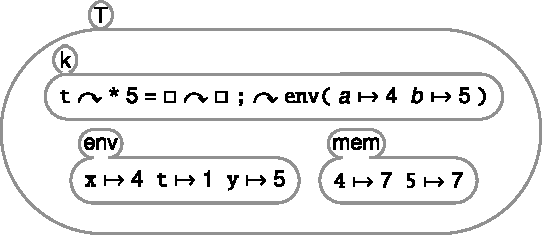
\includegraphics{figs/read-env-2}
\end{center}
\begin{minipage}{.44\columnwidth}
\begin{flushright}
cell comprehension
\end{flushright}
\end{minipage}
{\Huge$\mbox{\normalsize}\Downarrow\mbox{\normalsize }$}
\begin{minipage}{.44\columnwidth}
in-place rewriting
\end{minipage}
\begin{center}
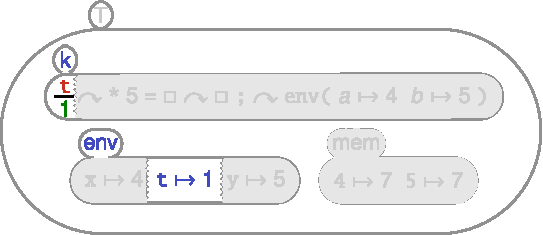
\includegraphics{figs/read-env2}
\end{center}
\begin{minipage}{.44\columnwidth}
\begin{flushright}
configuration abstraction
\end{flushright}
\end{minipage}
{\Huge$\mbox{\normalsize}\Downarrow\mbox{\normalsize }$}
\begin{minipage}{.44\columnwidth}
generalization
\end{minipage}
\[
\Kprefix{white}{k}{\reduce{\color{red}X}{\color{green}{V}}}\mathrel{}\Kmiddle{white}{env}{X\mapsto V}
\]
\caption{From running configurations to \K rules}\label{fig:k-rules}
\end{figure}

Figure~\ref{fig:k-rules} shows how the \K rule for reading the value of a local variable from the environment can be derived directly from the running configuration in which evaluating a local variable is the next task.  First, through a process named {\em cell comprehension} we focus only on the parts of the cells which are relevant for this rule.  At the same time, we can declare our intention to replace $t$ by its value in the environment (which is $1$) by underlining the part that needs to change and writing its replacement under the line, through what we call {\em in-place rewriting}.  Finally, through the process of {\em configuration abstraction}, only the relevant cells are kept, and through {\em generalization} we replace the concrete instances of identifiers and constants with variables of corresponding types.  The jagged edges are used to specify that there could be more content in the cell in addition to what is explicitly specified

The thus obtained \K rule succinctly describes the intuitive semantics for reading a local variable:  if a local variable $X$ is the next thing to be evaluated and if $X$ is mapped to a value $V$ in the environment, then replace that occurence of $X$ by $V$.  Moreover, it does that by only specifying what is needed from the configuration,  which is essential for obtaining modular definitions, and by precisely identifying what changes, which significantly enhances the concurrency.

\paragraph{Modularity.}  As mentioned above the configuration abstraction process is instrumental in achieving the desired modularity goal for the \K framework.  Relying on the initial configuration being specified by the designer, and the fact that usually the structure of such an configuration does not change during the execution of a program, the \K rules are essentially invariant under change of structure.  This effectively means that the same rule can be re-used in different definitions as long as the required cells are present, regardless or the additional context, which can be automatically inferred from the initial configuration.   As an example, the \K rule for reading the value of a local variable can be used for a configuration as the one specified above, for the full {\sc KernelC} configuration, and even for a configuration in which the computation and the environment cells are in separate parts of the configuration like in the following case:
\[\mallLarge{white}{T}{
 \mall{white}{thread}{
 {\color{blue!50!black}\mall{white}{k}{\color{black!25}
{{{{{{{{{\color{red!50!black}{\terminal{t}}}}\kra{{\terminal{*}{5}} \terminal{=} {\Hole}}}}}\kra{{\Hole}\terminal{;}}}}}\mathrel{{\kra}}{{\terminal{env(} {{a\mapsto 4}\mathrel{}{b\mapsto 5}}\terminal{)}}}}}}}
\kBR
\mall{white}{state}{
{\color{blue!50!black}\mall{white}{env}{\color{black!25}{{{{\terminal{x}}\mapsto 4}\mathrel{}{\color{blue!50!black}{\terminal{t}}\mapsto 1}\mathrel{}{{\terminal{y}}\mapsto 5}}}}}\mathrel{}{\mall{white}{mem}{\color{black!25}{{\terminal{4}}\mapsto 7}\mathrel{}{{\terminal{5}}\mapsto {{7}}}}}}
}
\]

\paragraph{Power of expression.} The structure of the computations, and the fact that the current task is always at the top of the computation as a similar effect on the power of expression, as configuration abstraction has for modularity.  Let us give some examples of the easiness to define in \K constructs which are known to be hard in other frameworks, thus arguing that the \K framework reached the expressibility goal for an ideal definitional framework.

One first such example is the control intensive call with current continuation (call/cc), which is present in several functional languages (like Scheme), and to some extent, even in some imperative programming languages (such as the long-jump construct in C).  Call/cc is known to be hard to capture in most frameworks (except reduction semantics with evaluation contexts) due to lack of access to execution context, which is there captured by the logical context, which lives at a meta-level which is not observable in the framework.  Having the entire remainder of computation always following the current redex, allows \K to capture this construct in a simple and succinct manner by the following two rules:
%\tworules{ 
\rkrule{Passing computation as value}{\ensuremath \mall{white}{k}{{{\reduce{{\terminal{callcc}{\variable{V}}}}{{{\variable{V}}\mathrel{}{{{\it cc}({\variable{K}})}}}}}\mathrel{\terminal{\ensuremath{\kra}}}{\variable{K}}}}}
%}{
 \rkrule{Applying computation as function}{\ensuremath \mall{white}{k}{\reduce{{{{{{{\it cc}({\variable{K}})}}\mathrel{}{\variable{V}}}}\mathrel{\terminal{\ensuremath{\kra}}}{\AnyVar}}}{{{\variable{V}}\mathrel{\terminal{\ensuremath{\kra}}}{\variable{K}}}}}}
% }

The first rule wraps the current reminder of the computation as a value and passes it to the argument of ``{\tt callcc}'', which is supposed to evaluate to a function.  If during the evaluation of that function call, the continuation value is applied to some value, then the reminder of the computation at that time is replaced by the saved computation to which the passed value is prefixed (as the result of the original {\tt callcc} expression).

% Another feature which is hard to represent in other frameworks is handling multiple tasks at the same time, as when defining synchronous communication, for example.  Although SOS-based frameworks can capture specific versions of feature for languages like CCS or pi-caculus, they can only do it there because the communication commands are always at the top of their processes.  \K computation's structure is again instrumental here, as it allows to easily match two redexes at the same time, as shown by the following rule, defining synchronous message passing in a multi-agent environment:
% \[{{\mmiddle{white}{agent}{{{\mall{white}{me}{\color{green!25!black}{\variable{N\ensuremath{\nothing_{1}}}}}}\mathrel{\terminal{}}{\mprefix{white}{k}{\reduce{{\terminal{sendSynch}{\variable{V}}\terminal{to}{\color{blue!25!black}{\variable{N\ensuremath{\nothing_{2}}}}}}}{\constant{\ensuremath{\terminal{skip}}}}}}}}}\mathrel{\terminal{}}{\mmiddle{white}{agent}{{{\mall{white}{me}{\color{blue!25!black}{\variable{N\ensuremath{\nothing_{2}}}}}}\mathrel{\terminal{}}{\mprefix{white}{k}{\reduce{\constant{\ensuremath{\terminal{receiveFrom}{\color{green!25!black}{\variable{N\ensuremath{\nothing_{1}}}}}}}}{\variable{V}}}}}}}}\]

% \noindent Reading the rule one can easily get the intended semantics:  if one agent, identified by $N_1$ attempts to send a message to an agent identified by $N_2$, and if that agent is waiting to receive a message from $N_1$, then the send construct is dissolved in the first agent, while the receive expression is replaced by the value being send in the receiver agent.

We cannot conclude the survey on the expressivity of the \K framework without mentioning its reflective capabilities.  Based on the fact that \K regards all computational tasks as being abstract syntax trees, all language constructs become labels applied to other ASTs; for example the expression $a+3$ is represented in \K as \(\_+\_(a(\bdot_{\it\color{black!25} List\{K\}}) \mathrel{\textit{\LARGE\(,\)}}3(\bdot_{\it\color{black!25} List\{K\}}))\).  This abstract view of syntax allows reducing the computation-creating constructs to the following minimal core:

\medskip
\syntax{\nonTerminal{\sort{K}}}{\nonTerminal{\sort{KLabel}} ( \nonTerminal{\sort{List\{K\}}} )}{} 
\syntaxContt{\nonTerminal{\sort{K}}}{\bdot_{\color{black!25}K}}{} 
\syntaxContt{\nonTerminal{\sort{K}}}{K \kra K}{} 
\syntax{\nonTerminal{\sort{List\{K\}}}}{K}{}
\syntaxContt{\nonTerminal{\sort{List\{K\}}}}{\bdot_{\it List\{K\}}}{}
\syntaxContt{\nonTerminal{\sort{List\{K\}}}}{\nonTerminal{\sort{List\{K\}}}\mathrel{\textit{\LARGE\(,\)}}\nonTerminal{\sort{List\{K\}}}}{}

\medskip
\noindent Moreover, this approach allows one to define a generic AST visitor, and in turn use that to define powerful reflective features such as code generation or a binder-independent substitution.  

% \paragraph{Concurrency.}  Another feature that makes \K a really good choice for defining programming languages is its natural way of capturing concurrency.  Besides being truely concurrent as the chemical abstract machine, and thus matching the goals set above for an ideal framework, \K rules also allow capturing concurrency with sharing of resources.

% Let us exemplify this concurrency power.  The two rules specified below are the {\sc KernelC} rules for accessing/updating the value at a memory location:

% \begin{minipage}{.4\columnwidth}
% \kkrule{}{\ensuremath{{\bprefix{white}{k}{\reduce{{\color{red!25!black}{\terminal{*}{\variable{N}}}\terminal{=}{\variable{V}}}}{\color{green!25!black}\variable{V}}}}\mathrel{\terminal{}}{\bmiddle{white}{mem}{{{\variable{N}}\mathrel{\terminal{\ensuremath{\mapsto}}}{\color{black}\reduce{{\color{red!25!black}\bAnyVar}}{\color{green!25!black}\variable{V}}}}}}}}
% \end{minipage}\hfill
% \begin{minipage}{.3\columnwidth}
% \kkrule{}{\ensuremath{{\bprefix{white}{k}{\reduce{{\color{red!25!black}\terminal{*}{\variable{N}}}}{\color{green!25!black}\variable{V}}}}\mathrel{\terminal{}}{\bmiddle{white}{mem}{{{\variable{N}}\mathrel{\terminal{\ensuremath{\mapsto}}}{\variable{V}}}}}}}
% \end{minipage}%

% Consider first a configuration where two threads, symbolized by two computation cells, are both ready to read the value of the same memory location:  

% \noindent\(
% \ball{white}{T}{
% \begin{array}{c}
% {\ball{white}{k}{{{\color{red!25!black}\terminal{*}{\variable{3}}}}\kra\cdots}}
% {\ball{white}{k}{{{\color{red!25!black}\terminal{*}{\variable{3}}}}\kra\cdots}}
% \kBR
% {\color{blue!25!black}\ball{white}{mem}{\color{black}{2\mapsto 5}\mathrel{}{\color{blue!25!black}{3\mapsto 1}}\mathrel{}{4\mapsto 6}}}
% \end{array}
% }
% \mbox{\LARGE$\ \skarrow{}$}
% \ball{white}{T}{
% \begin{array}{c}
% {\ball{white}{k}{{{\color{green!25!black}\constant{1}}}\kra\cdots}}
% {\ball{white}{k}{{{\color{green!25!black}\constant{1}}}\kra\cdots}}
% \kBR
% {\color{blue!25!black}\ball{white}{mem}{\color{black}{2\mapsto 5}\mathrel{}{\color{blue!25!black}{3\mapsto 1}}\mathrel{}{4\mapsto 6}}}
% \end{array}
% }
% \)

% As the semantics of the K rules specify that the parts of the configuration which are only read by the rule, can be shared by concurrent applications (here the memory cell construct and the mapping of location $3$ to value $1$),
% the read rule can match for both threads and they can both advance one step concurrently.


% A similar thing happens for concurrent updates.  As long as both threads attempt to update distinct locations, the update rules can match them both and they can advance concurrently:
% \[
% \ball{white}{T}{
% \begin{array}{c}
% \!\!{\ball{white}{k}{{{\color{red!25!black}{\terminal{*}{\variable{2}}}\terminal{=}9}}\kra\cdots\!\!}}
% {\ball{white}{k}{{{\color{red!25!black}{\terminal{*}{\variable{3}}}\terminal{=}0}}\kra\cdots\!\!}}\!\!\!
% \kBR
% {\color{blue!25!black}\ball{white}{mem}{\color{black}{{\color{blue!25!black}2\mapsto {\color{red!25!black}5}}}\mathrel{}{\color{blue!25!black}{3\mapsto {\color{red!25!black}1}}}\mathrel{}{4\mapsto 6}}}
% \end{array}
% }
% \mbox{\LARGE$\ \skarrow{}$}
% \ball{white}{T}{
% \begin{array}{c}
% {\ball{white}{k}{{{\color{green!25!black}{9}}}\kra\cdots\!\!}}
% {\ball{white}{k}{{{\color{green!25!black}{0}}}\kra\cdots\!\!}}
% \kBR
% \!\!\!{\color{blue!25!black}\ball{white}{mem}{\color{black}{{\color{blue!25!black}2\mapsto {\color{green!25!black}{9}}}}\mathrel{}{\color{blue!25!black}{3\mapsto {\color{green!25!black}{0}}}}\mathrel{}{4\mapsto 6}}}\!\!
% \end{array}
% }
% \]

% Moreover, by disallowing rule instances to overlap on the parts they change, the K semantics enforces sequentialization of dataraces, as shown in Figure~\ref{fig:dataraces}. 

% \begin{figure}
% \[
% \begin{array}{cc}
% \multicolumn{2}{c}{
% \ball{white}{T}{
% \begin{array}{c}
% {\ball{white}{k}{{{{{\terminal{*}{\variable{3}}}\terminal{=}0}}}\kra\cdots}}
% {\ball{white}{k}{{\terminal{*}{\variable{3}}}\kra\cdots}}
% \kBR
% {\ball{white}{mem}{{{2\mapsto {5}}}\mathrel{}{{3\mapsto {1}}}\mathrel{}{4\mapsto 6}}}
% \end{array}
% }}
% \\
% \rotatebox[origin=c]{-135}{\LARGE$\ \skarrow{}$}
% &
% \rotatebox[origin=c]{-45}{\LARGE$\ \skarrow{}$}
% \\
% \ball{white}{T}{
% \begin{array}{c}
% {\ball{white}{k}{{{0}}\kra\cdots}}
% {\ball{white}{k}{{\terminal{*}{\variable{3}}}\kra\cdots}}
% \kBR
% {\ball{white}{mem}{{{2\mapsto {5}}}\mathrel{}{{3\mapsto 0}}\mathrel{}{4\mapsto 6}}}
% \end{array}
% }
% &
% \ball{white}{T}{
% \begin{array}{c}
% {\ball{white}{k}{{{{{\terminal{*}{\variable{3}}}\terminal{=}0}}}\kra\cdots}}
% {\ball{white}{k}{1\kra\cdots}}
% \kBR
% {\ball{white}{mem}{{{2\mapsto {5}}}\mathrel{}{{3\mapsto {1}}}\mathrel{}{4\mapsto 6}}}
% \end{array}
% }
% \\
% \rotatebox[origin=c]{-90}{\LARGE$\ \skarrow{}$}
% &
% \rotatebox[origin=c]{-90}{\LARGE$\ \skarrow{}$}
% \\
% \ball{white}{T}{
% \begin{array}{c}
% {\ball{white}{k}{{{0}}\kra\cdots}}
% {\ball{white}{k}{0\kra\cdots}}
% \kBR
% {\ball{white}{mem}{{{2\mapsto {5}}}\mathrel{}{{3\mapsto 0}}\mathrel{}{4\mapsto 6}}}
% \end{array}
% }
% &
% \ball{white}{T}{
% \begin{array}{c}
% {\ball{white}{k}{{{0}}\kra\cdots}}
% {\ball{white}{k}{1\kra\cdots}}
% \kBR
% {\ball{white}{mem}{{{2\mapsto {5}}}\mathrel{}{{3\mapsto 0}}\mathrel{}{4\mapsto 6}}}
% \end{array}
% }
% \end{array}
% \]
% \caption{Dataraces are forced to sequentialize}\label{fig:dataraces}
% \end{figure}
%\section{Semantics}
\pagebreak
\section{C Semantics}
Here we present the full C semantics, generated directly from the original source code (which can be found on our Google project page at \url{https://code.google.com/p/k-framework/wiki/DefinitionOfC}).  The \LaTeX{} is being generated through a very new backend, and as such, there may be a number of typesetting/formatting or even correctness errors in the \LaTeX{}.  In particular, sometimes important parentheses have been discarded, which can change the meaning of side conditions.  If there is any doubt, please consult the original source code at the above URL.

Where made possible by the tool, the original abstract syntax is in \texttt{typewriter} font and the semantic syntax is in \textsf{sans-serif}.

\eject \pdfpagewidth=15in \pdfpageheight=9in
\includepdf[pages=1-,noautoscale=true,offset=3.25in 1.25in]{c.pdf}

\bibliography{refs}
\end{document}
